\hypertarget{introduction}{%
\section{Introduction}\label{introduction}}

The Kitaev-Honeycomb model is remarkable because it was the first such
model that combined three key properties.

First, it is a plausible tight binding Hamiltonian. The form of the
Hamiltonian could be realised by a real material. Indeed candidate
materials such as \(\alpha\mathrm{-RuCl}_3\) were quickly found
\autocite{banerjeeProximateKitaevQuantum2016,trebstKitaevMaterials2022}
that are expected to behave according to the Kitaev with small
corrections.

Second, the Kitaev Honeycomb model is deeply interesting to modern
condensed matter theory. Its ground state is almost the canonical
example of the long sought after quantum spin liquid state. Its
excitations are anyons, particles that can only exist in two dimensions
that break the normal fermion/boson dichotomy. Anyons have been the
subject of much attention because, among other reasons, there are
proposals to braid them through space and time to achieve noise tolerant
quantum computations
\textcite{freedmanTopologicalQuantumComputation2003}.

Third and perhaps most importantly, it a rare many body interacting
quantum system that can be treated analytically. It is exactly
solveable. We can explicitly write down its many body ground states in
terms of single particle states
\textcite{kitaevAnyonsExactlySolved2006}. Its solubility comes about
because the model has extensively many conserved degrees of freedom that
mediate the interactions between quantum degrees of freedom.

In this chapter I will discuss the physics of the Kitaev Model on
amorphous lattices.

I'll start by discussing the physics of the Kitaev model in much more
detail. Here I will look at the gauge symmetries of the model as well as
its solution via a transformation to a Majorana hamiltonian. From this
discusssion we will see that for the the model to be sovleable it need
only be defined on a trivalent, tri-edge-colourable lattice
\autocite{Nussinov2009}.

In the methods section, I will discuss how to generate such lattices and
colour them as well as how to map back and forth between configurations
of the gauge field and configurations of the gauge invariant quantities.

In results section, I will begin by looking at the zero temperature
physics. I'll present numerical evidence that the ground state of the
model is given by a simple rule. I'll make an assessment of the gapless,
abelian and non-abelian phases that are present as well as spontaneous
chiral symmetry breaking and topological edge states. We will also
compare the zero temperature phase diagram to that of the Kitaev
Honeycomb Model. Next I will take the model to finite temperature and
demonstrate that there is a phase transition to a thermal metal state.

In the Discussion I will consider possible physical realisations of this
model as well the motivations for doing so. I will alao discuss how a
well known quantum error correcting code defined on the Kitaev Honeycomb
could be generalised to the amorphous case.

Various generalisations have been made, one mode replaces pairs of
hexagons with heptagons and pentagons
\cite{periNonAbelianChiralSpin2020} and another that replaces vertices
of the hexagons with triangles \cite{yaoExactChiralSpin2007}. When we
generalise this to the amorphous case, the key property that will remain
is that each vertex interacts with exactly three others via an x, y and
z edge. However the lattice will no longer be bipartite, breaking chiral
symmetry among other things.

Kitaev-Heisenberg Model In real materials there will generally be an
addtional small Heisenberg term
\[H_{KH} =  - \sum_{\langle j,k\rangle_\alpha} J^{\alpha}\sigma_j^{\alpha}\sigma_k^{\alpha} + \sigma_j\sigma_k\]

\hypertarget{amorphous-systems}{%
\subsection{Amorphous Systems}\label{amorphous-systems}}

\textbf{Insert discussion of why a generalisation to the amorphous case
is intersting}

\hypertarget{the-kitaev-model}{%
\subsection{The Kitaev Model}\label{the-kitaev-model}}

\hypertarget{commutation-relations}{%
\subsubsection{Commutation relations}\label{commutation-relations}}

Before diving into the Hamiltonian of the Kitaev Model, here is a quick
refresher of the key commutation relations of spins, fermions and
Majoranas.

\hypertarget{spins}{%
\paragraph{Spins}\label{spins}}

Skip this is you're super familiar with the algebra of the Pauli
martrices. Scalars like \(\delta_{ij}\) should be understood to be
multiplied by an implicit identity \(\mathbb{1}\) where necessary.

We can represent a single spin\(-1/2\) particle using the Pauli matrices
\((\sigma^x, \sigma^y, \sigma^z) = \vec{\sigma}\), these matrices all
square to the identity \(\sigma^\alpha \sigma^\alpha = \mathbb{1}\) and
obey nice commutation and exchange rules:
\[\sigma^\alpha \sigma^\beta = \delta^{\alpha \beta} + i \epsilon^{\alpha \beta \gamma} \sigma^\gamma\]
\[[\sigma^\alpha, \sigma^\beta] = 2 i \epsilon^{\alpha \beta \gamma} \sigma^\gamma\]

Adding a sites indices \(ijk...\), spins at different spatial sites
commute always \([\vec{\sigma}_i, \vec{\sigma}_j] = 0\) so when
\(i \neq j\)
\[\sigma_i^\alpha \sigma_j^\beta = \sigma_j^\alpha \sigma_i^\beta\]
\[[\sigma_i^\alpha, \sigma_j^\beta] = 0\] while the previous equations
hold for \(i = j\).

Two extra relations that will be useful for the Kitaev model are the
value of \(\sigma^\alpha \sigma^\beta \sigma^\gamma\) and
\([\sigma^\alpha \sigma^\beta, \sigma^\gamma]\) when
\(\alpha \neq \beta \neq \gamma\) these can be computed quite easily by
appling the above relations yielding:
\[\sigma^\alpha \sigma^\beta \sigma^\gamma = i \epsilon^{\alpha\beta\gamma}\]
and \[[\sigma^\alpha \sigma^\beta, \sigma^\gamma] = 0\]

\hypertarget{fermions-and-majoranas}{%
\paragraph{Fermions and Majoranas}\label{fermions-and-majoranas}}

The fermionic creation and anhilation operators are defined by the
canonical anticommutation relations \[\begin{aligned}
\{f_i, f_j\} &= \{f^\dagger_i, f^\dagger_j\} = 0\\
\{f_i, f^\dagger_j\} &= \delta_{ij}
\end{aligned}\] which give us the exchange statistics and Pauli
exclusion principle.

From fermionic operators, we can construct Majorana operators:
\[\begin{aligned}
f_i         &= 1/2 (a_i + ib_i)\\
f^\dagger_i &= 1/2(a_i - ib_i)\\
a_i         &= f_i + f^\dagger_i = 2\mathbb{R}f\\
b_i         &= 1/i(f_i - f^\dagger_i) = 2\mathbb{I} f 
\end{aligned}\]

Majorana operators are the real and imaginary parts of the fermionic
operators, physically they correspond to the orthogonal superpositions
of the presence and absence of the fermion and are thus a kind of
quasiparticle.

Once we involve multiple fermions there is quite a bit of freedom in how
we can perform the transformation from \(n\) fermions \(f_i\) to \(2n\)
Majoranas \(c_i\). The property that must be preserved however is that
the Majoranas still anticommute:

\[ \{c_i, c_j\} = 2\delta_{ij}\]

\hypertarget{the-hamiltonian}{%
\subsubsection{The Hamiltonian}\label{the-hamiltonian}}

To get down to brass tacks, the Kitaev Honeycomb model is a model of
interacting spin\(-1/2\)s on the vertices of a honeycomb lattice. Each
bond in the lattice is assigned a label \(\alpha \in \{ x, y, z\}\) and
that bond couples its two spin neighbours along the \(\alpha\) axis. See
\cref{fig:visual_kitaev_1} for a diagram.

This gives us the Hamiltonian
\[H =  - \sum_{\langle j,k\rangle_\alpha} J^{\alpha}\sigma_j^{\alpha}\sigma_k^{\alpha},\]
where \(\sigma^\alpha_j\) is a Pauli matrix acting on site \(j\) and
\(\langle j,k\rangle_\alpha\) is a pair of nearest-neighbour indices
connected by an \(\alpha\)-bond with exchange coupling \(J^\alpha\)
\textcite{kitaevAnyonsExactlySolved2006}. For notational brevity is is
useful to introduce the bond operators
\(K_{ij} = \sigma_j^{\alpha}\sigma_k^{\alpha}\) where \(\alpha\) is a
function of \(i,j\) that picks the correct bond type.

\begin{figure}
\hypertarget{fig:visual_kitaev_1}{%
\centering
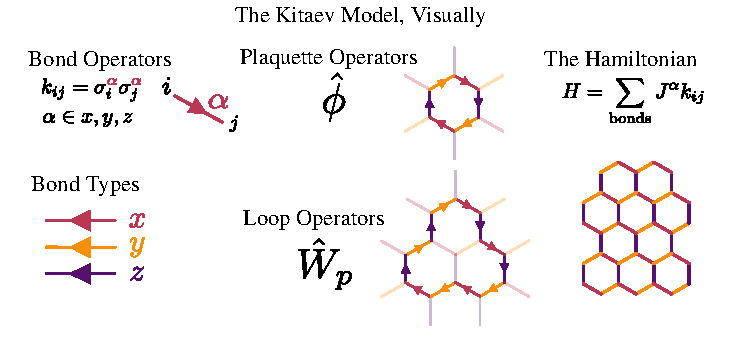
\includegraphics[width=1\textwidth,height=\textheight]{figure_code/amk_chapter/visual_kitaev_1.pdf}
\caption{}\label{fig:visual_kitaev_1}
}
\end{figure}

This Kitaev model has a set of conserved quantities that, in the spin
language, take the form of Wilson loop operators \(W_p\) winding around
a closed path on the lattice. The direction doesn't matter, but I will
stick to clockwise here. I'll use the term plaquette and the symbol
\(\phi\) to refer to a Wilson loop operator that does not enclose any
other sites, such as a single hexagon in a honeycomb lattice.

\[W_p = \prod_{\mathrm{i,j}\; \in\; p} K_{ij} = \sigma_1^z \sigma_2^x \sigma_2^y \sigma_3^y .. \sigma_n^y \sigma_n^y \sigma_1^z\]

\textbf{add a diagram of a single plaquette with labelled site and bond
types}

In closed loops, each site appears twice in the product with two of the
three bond types. Applying
\(\sigma^\alpha \sigma^\beta = \epsilon^{\alpha \beta \gamma} \sigma^\gamma, \alpha \neq \beta\)
then gives us a product containing a single pauli matrix associated with
each site in the loop with the type of the \emph{outward} pointing bond.
From this we see that the \(W_p\) associated with hexagons or shapes
with an even number of sides all square to 1 and hence have eigenvalues
\(\pm 1\).

A consequence of the fact that the honeycomb lattice is bipartite is
that there are no closed loops that contain an even number of
edges\footnote{A bipartite lattice is composed of A and B sublattices
  with no intra-sublattice edges i.e no A-A or B-B edges. Any closed
  loop must begin and at the same site, let's say it's an A site. The
  loop must go A-B-A-B\ldots{} until it returns to the original site and
  must therefore must contain an even number of edges in order to end on
  the same sublattice that it started on.} and hence all the \(W_p\)
have eigenvalues \(\pm 1\) on bipartite lattices. Later we will show
that plaquettes with an odd number of sides (odd plaquettes for short)
will have eigenvalues \(\pm i\).

\begin{figure}
\hypertarget{fig:regular_plaquettes}{%
\centering
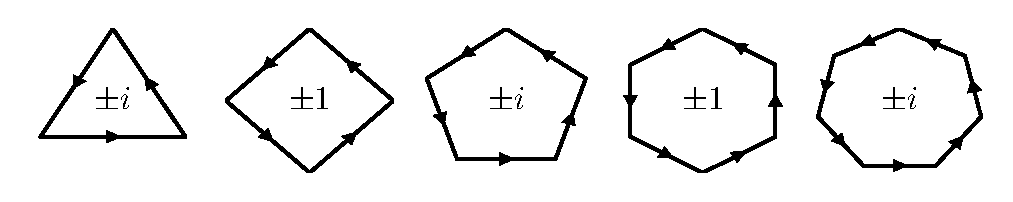
\includegraphics[width=0.86\textwidth,height=\textheight]{figure_code/amk_chapter/regular_plaquettes/regular_plaquettes.pdf}
\caption{The eigenvalues of a loop or plaquette operators depend on how
many bonds in its enclosing path.}\label{fig:regular_plaquettes}
}
\end{figure}

Remarkably, all of the spin bond operators \(K_{ij}\) commute with all
the Wilson loop operators \(W_p\). \[[W_p, J_{ij}] = 0\] We can prove
this by considering the three cases: 1. neither \(i\) nor \(j\) is part
of the loop 2. one of \(i\) or \(j\) are part of the loop 3. both are
part of the loop

The first case is trivial while the other two require a bit of algebra,
outlined in \cref{fig:visual_kitaev_2}.

\begin{figure}
\hypertarget{fig:visual_kitaev_2}{%
\centering
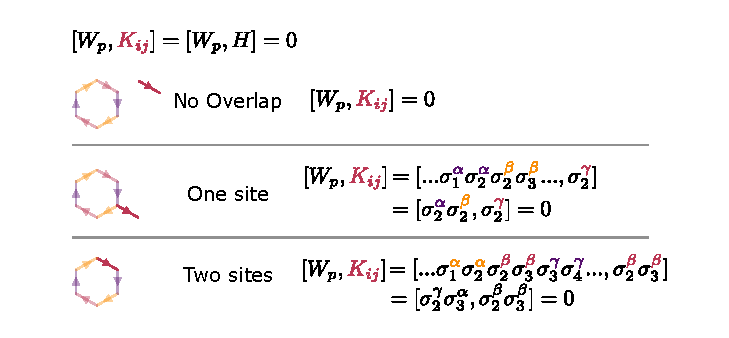
\includegraphics[width=1.43\textwidth,height=\textheight]{figure_code/amk_chapter/visual_kitaev_2.pdf}
\caption{}\label{fig:visual_kitaev_2}
}
\end{figure}

Since the Hamiltonian is just a linear combination of bond operators, it
also commutes with the plaquette operators! This is great because it
means that the there's a simultaneous eigenbasis for the Hamiltonian and
the plaquette operators. We can thus work in a basis in which the
eigenvalues of the plaquette operators take on a definite value and for
all intents and purposes act like classical degrees of freedom. These
are the extensively many conserved quantities that make the model
tractable.

Plaquette operators measure flux. We will find that the ground state of
the model corresponds to some particular choice of flux through each
plaquette. I will refer to excitations which flip the expectation value
of a plaqutte operator away from the ground state as \textbf{vortices}.

Fixing a configuration of the vortices thus partitions the many-body
Hilbert space into a set of `vortex sectors' labelled by that particular
flux configuration \(\phi_i = \pm 1,\pm i\).

\hypertarget{from-spins-to-majorana-operators}{%
\subsubsection{From Spins to Majorana
operators}\label{from-spins-to-majorana-operators}}

\hypertarget{for-a-single-spin}{%
\paragraph{For a single spin}\label{for-a-single-spin}}

Let's start by considering just one site and its \(\sigma^x, \sigma^y\)
and \(\sigma^z\) operators which live in a two dimensional Hilbert space
\(\mathcal{L}\).

We will introduce two fermionic modes \(f\) and \(g\) that satisy the
canonical anticommutation relations along with their number operators
\(n_f = f^\dagger f, n_g = g^\dagger g\) and the total fermionic parity
operator \(F_p = (2n_f - 1)(2n_g - 1)\) which we can use to divide their
Fock space up into even and odd parity subspaces which are separated by
the addition or removal of one fermion.

From these two fermionic modes we can build four Majorana operators:
\[\begin{aligned}
b^x &= f + f^\dagger\\
b^y &= -i(f - f^\dagger)\\
b^z &= g + g^\dagger\\
c   &= -i(g - g^\dagger)
\end{aligned}\]

The Majoranas obey the usual commutation relations, squaring to one and
anticommuting with eachother. The fermions and Majorana live in a 4
dimenional Fock space \(\mathcal{\tilde{L}}\). We can therefore identify
the two dimensional space \(\mathcal{M}\) with one of the partity
subspaces of \(\mathcal{\tilde{L}}\) which we will call the
\emph{physical subspace} \(\mathcal{\tilde{L}}_p\). Kitaev defines the
operator \[D = b^xb^yb^zc\] which can be expanded out to
\[D = -(2n_f - 1)(2n_g - 1) = -F_p\] and labels the physical subspace as
the space sanned by states for which \[ D|\phi\rangle = |\phi\rangle\]

We can also think of the physical subspace as whatever is left after
applying the projector \[P  = \frac{1 - D}{2}\] to it. This formulation
will be useful for taking states that span the extended space
\(\mathcal{\tilde{M}}\) and projecting them into the physical subspace.

So now, with the caveat that we are working in the physical subspace, we
can define new pauli operators:

\[\tilde{\sigma}^x = i b^x c,\; \tilde{\sigma}^y = i b^y c,\; \tilde{\sigma}^y = i b^y c\]

These extended space pauli operators satisfy all the usual commutation
relations, the only difference being that if we evaluate
\(\sigma^x \sigma^y \sigma^z = i\) we instead get
\[ \tilde{\sigma}^x\tilde{\sigma}^y\tilde{\sigma}^z = iD \]

Which indeed makes sense, as long as we promise to confine ourselves to
the physical subspace \(D = 1\) and this all makes sense.

\begin{figure}
\hypertarget{fig:majorana}{%
\centering
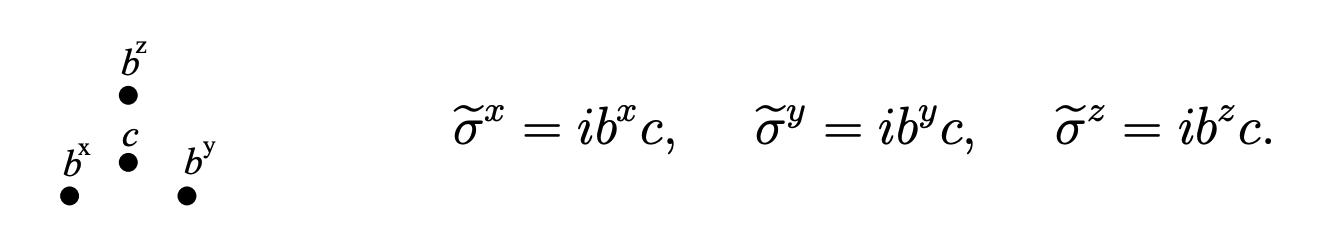
\includegraphics[width=0.71\textwidth,height=\textheight]{figure_code/majorana.png}
\caption{}\label{fig:majorana}
}
\end{figure}

\hypertarget{for-multiple-spins}{%
\paragraph{For multiple spins}\label{for-multiple-spins}}

This construction generalises easily to the case of multiple spins: we
get a set of 4 Majoranas \(b^x_j,\; b^y_j,\;b^z_j,\; c_j\) and a
\(D_j = b^x_jb^y_jb^z_jc_j\) operator for every spin. For a state to be
physical we require that \(D_j |\psi\rangle = |\psi\rangle\) for all
\(j\).

From these each Pauli operator can be constructed:
\[\tilde{\sigma}^\alpha_j = i b^\alpha_j c_j\]

This is where the magic happens. We can promote the spin hamiltonian
from \(\mathcal{L}\) into the extended space \(\mathcal{\tilde{L}}\),
safe in the knowledge that nothing changes so long as we only actually
work with physical states. The Hamiltonian \[\begin{aligned}
\tilde{H} &=  - \sum_{\langle j,k\rangle_\alpha} J^{\alpha}\tilde{\sigma}_j^{\alpha}\tilde{\sigma}_k^{\alpha}\\
          &= \frac{i}{4} \sum_{\langle j,k\rangle_\alpha} 2J^{\alpha} (ib^\alpha_i b^\alpha_j) c_i c_j\\
          &=  \frac{i}{4} \sum_{\langle i,j\rangle_\alpha} 2J^{\alpha} \hat{u}_{ij} \hat{c}_i \hat{c}_j
\end{aligned}\]

We can factor out the Majorana bond operators
\(\hat{u}_{ij} = i b^\alpha_i b^\alpha_j\). Note that these bond
operators are not equal to the spin bond operators
\(K_{ij} = \sigma^\alpha_i \sigma^\alpha_j = - \hat{u}_{ij} c_i c_j\).
In what follows we will work much more frequently with the Majorana bond
operators so when I refer to bond operators without qualification, I am
refering to the Majorana variety.

Similar to the argument with the spin bond operators \(K_{ij}\) we can
quickly verify by considering three cases that the Majorana bond
operators \(u_{ij}\) all commute with one another. They square to one so
have eigenvalues \(\pm 1\) and they also commute with the \(c_i\)
operators.

Another important point here is that the operators
\(D_i = b^x_i b^y_i b^z_i c_i\) commute with \(K_{ij}\) and therefore
with \(\tilde{H}\). We will show later that the action of \(D_i\) on a
state is to flip the values of the three \(u_{ij}\) bonds that connect
to site \(i\). Physcially this is telling us that \(u_{ij}\) is a gauge
field with a high degree of degeneracy.

In summary Majorana bond operators \(u_{ij}\) are an emergent,
classical, \(\mathbb{Z_2}\) gauge field!

\hypertarget{partitioning-the-hilbert-space-into-bond-sectors}{%
\subsubsection{Partitioning the Hilbert Space into Bond
sectors}\label{partitioning-the-hilbert-space-into-bond-sectors}}

Similar to the story with the plaquette operators from the spin
language, we can break the Hilbert space \(\mathcal{L}\) up into sectors
labelled by the a set of choices \(\{\pm 1\}\) for the value of each
\(u_{ij}\) operator which I denote by \(\mathcal{L}_u\). Since
\(u_{ij} = -u_{ji}\) we can represent the \(u_{ij}\) graphically with an
arrow that points along each bond in the direction in which
\(u_{ij} = 1\).

Once confined to a particular \(\mathcal{L}_u\), we can `remove the
hats' from the \(\hat{u}_{ij}\) and the hamiltonian becomes a quadratic,
free fermion problem
\[\tilde{H_u} =  \frac{i}{4} \sum_{\langle i,j\rangle_\alpha} 2J^{\alpha} u_{ij} c_i c_j\]
the ground state of which, \(|\psi_u\rangle\) can be found easily via
matrix diagonalisation. If you have been paying very close attention,
you may at this point ask whether the \(\mathcal{L}_u\) are confined
entirely within the physical subspace \(\mathcal{L}_p\) and indeed we
will see that they are not. However it will be helpful to first develop
the theory of the Majorana Hamiltonian a little more.

\begin{figure}
\hypertarget{fig:intro_figure_template}{%
\centering
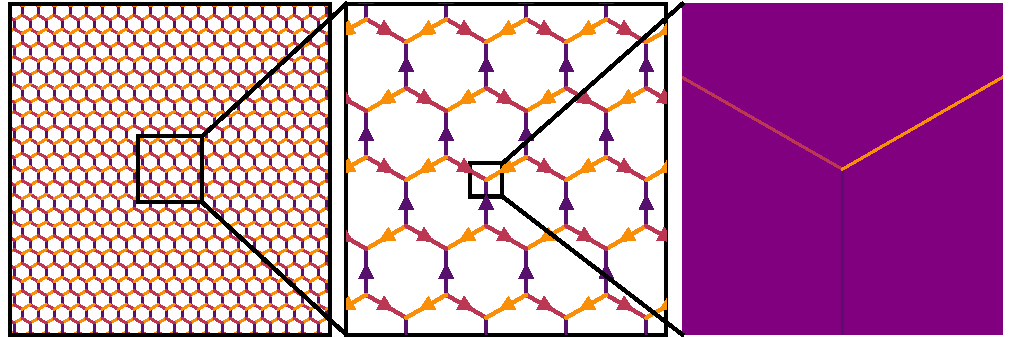
\includegraphics[width=1\textwidth,height=\textheight]{figure_code/amk_chapter/honeycomb_zoom/intro_figure_template.pdf}
\caption{\textbf{(a)} The standard Kitaev Model is defined on a
honeycomb lattice. The special feature of the honeycomb lattice that
makes the model solveable it is that each vertex is joined by exactly
three bonds i.e the lattice is trivalent. One of three labels is
assigned to each \textbf{(b)} We represent the antisymmetric gauge
degree of freedom \(u_{jk} = \pm 1\) with arrows that point in the
direction \(u_{jk} = +1\) \textbf{(c)} The Majorana transformation can
be visualised as breaking each spin into four Majoranas which then pair
along the bonds. The pairs of x,y and z Majoranas become part of the
classical \(\mathbb{Z}_2\) gauge field \(u_{ij}\) leaving just a single
Majorana \(c_i\) per site.}\label{fig:intro_figure_template}
}
\end{figure}

\hypertarget{the-majorana-hamiltonian}{%
\subsection{The Majorana Hamiltonian}\label{the-majorana-hamiltonian}}

We now have a quadtratic hamiltonian
\[ \tilde{H} =  \frac{i}{4} \sum_{\langle i,j\rangle_\alpha} 2J^{\alpha} u_{ij} c_i c_j\]
in which most of the Majorana degrees of freedom have paired along bonds
to become a classical gauge field \(u_{ij}\). What follows is relatively
standard theory for quadratic Majorana Hamiltonians
\textcite{BlaizotRipka1986}.

As a consequence of the the antisymmetry of the matrix with entries
\(J^{\alpha} u_{ij}\), the eigenvalues of the Hamiltonian
\(\tilde{H}_u\) come in pairs \(\pm \epsilon_m\). This redundant
information is a consequence of the doubling of the Hilbert space which
occured when we transformed to the Majorana representation.

If we pair organise the eigenmodes of \(H\) into pairs such that \(b_m\)
and \(b_m'\) have energies \(\epsilon_m\) and \(-\epsilon_m\) we can
construct the transformation \(Q\)
\[(c_1, c_2... c_{2N}) Q = (b_1, b_1', b_2, b_2' ... b_{N}, b_{N}')\]
and put the Hamiltonian into the form
\[\tilde{H}_u = \frac{i}{2} \sum_m \epsilon_m b_m b_m'\]

The determinant of \(Q\) will be useful later when we consider the
projector from \(\mathcal{\tilde{L}}\) to \(\mathcal{L}\) but otherwise
the \(b_m\) are just an intermediate step. From them we form fermionic
operators \[ f_i = \tfrac{1}{2} (b_m + ib_m')\] with their associated
number operators \(n_i = f^\dagger_i f_i\). These let us write the
Hamiltonian neatly as

\[ \tilde{H}_u = \sum_m \epsilon_m (n_m - \tfrac{1}{2}).\]

The ground state \(|n_m = 0\rangle\) of the many body system at fixed
\(u\) is then \[E_{u,0} = -\frac{1}{2}\sum_m \epsilon_m \] and we can
construct any state from a particular choice of \(n_m = 0,1\).

In cases where all we care about it the value of \(E_{u,0}\) it is
possible to skip forming the fermionic operators. The eigenvalues
obtained directly from diagonalising \(J^{\alpha} u_{ij}\) come in
\(\pm \epsilon_m\) pairs. We can take half the absolute value of the
whole set to recover \(\sum_m \epsilon_m\) easily.

\textbf{The Majorana Hamiltonian is quadratic within a Bond Sector.}

\hypertarget{mapping-back-from-bond-sectors-to-the-physical-subspace}{%
\subsubsection{Mapping back from Bond Sectors to the Physical
Subspace}\label{mapping-back-from-bond-sectors-to-the-physical-subspace}}

At this point, given a particular bond configuration \(u_{ij} = \pm 1\)
we are able to construct a quadratic Hamiltonian \(\tilde{H}_u\) in the
extended space and diagonalise it to find its ground state
\(|\vec{u}, \vec{n} = 0\rangle\). This is not necessarily the ground
state of the system as a whole, it just the lowest energy state within
the subspace \(\mathcal{L}_u\)

\textbf{However, \(|u, n_m = 0\rangle\) does not lie in the physical
subspace}. As an example let's take the lowest energy state associated
with \(u_{ij} = +1\), this state satisfies
\[u_{ij} |\vec{u}=1, \vec{n} = 0\rangle = |\vec{u}=1, \vec{n} = 0\rangle\]
for all bonds \(i,j\).

If we act on it this state with one of the gauge operators
\(D_j = b_j^x b_j^y b_j^z c_j\) we see that \(D_j\) flips the value of
the three bonds \(u_{ij}\) that surround site \(k\):

\[ |u'\rangle = D_j |u=1, n_m = 0\rangle\]

\[ \begin{aligned}
\langle u'|u_{ij}|u'\rangle &=  \langle u| b_j^x b_j^y b_j^z c_j \;ib^x_i b^x_j\; b_j^x b_j^y b_j^z c_j|u\rangle\\
&= -1
\end{aligned}\]

Since \(D_j\) commutes with the hamiltonian in the extended space
\(\tilde{H}\), the fact that \(D_j\) flips the value of bond operators
is telling us that there is a gauge degeneracy between the ground state
of \(\tilde{H}_u\) and the set of \(\tilde{H}_{u'}\) related to it by
gauge transformations \(D_j\). I.e we can flip any three bonds around a
vertex and the physics will stay the same.

We can turn this into a symmetrisation procedure by taking a
superposition of every possible gauge transformation. Every possible
gauge transformation is just every possible subset of
\({D_0, D_1 ... D_n}\) which can be neatly expressed as
\[|\phi_w\rangle = \prod_i \left( \frac{1 + D_i}{2}\right) |\tilde{\phi}_u\rangle\]
this is nice because the quantity \(\frac{1 + D_i}{2}\) is also the
local projector onto the physical subspace. Here \(|\phi_w\rangle\) is a
gauge invariant state that lives in \(\mathcal{L}_p\) which has been
constructed from a set of states in different \(\mathcal{L}_u\).

This gauge degeneracy leads nicely onto the next topic which is how to
construct a set of gauge invariant quantities out of the \(u_{ij}\),
these will turn out to just be the plaquette operators.

\textbf{The Bond Sectors overlap with the physical subspace but are not
contained within it.}

\hypertarget{open-boundary-conditions}{%
\subsubsection{Open boundary
conditions}\label{open-boundary-conditions}}

Care must be taken in the definition of open boundary conditions. Simply
removing bonds from the lattice leaves behind unpaired \(b^\alpha\)
operators that need to be paired in some way to arrive at fermionic
modes. In order to fix a pairing we always start from a lattice defined
on the torus and generate a lattice with open boundary conditions by
defining the bond coupling \(J^{\alpha}_{ij} = 0\) for sites joined by
bonds \((i,j)\) that we want to remove. This creates fermionic zero
modes \(u_{ij}\) associated with these cut bonds which we set to 1 when
calculating the projector.

Alternatively, since all the fermionic zero modes are degenerate anyway,
an arbitrary pairing of the unpaired \(b^\alpha\) operators could be
performed. \textbf{Is is possible that a lattice constructed and
coloured like this would have unequal numbers of \(b^x\) \(b^y\) and
\(b^z\) operators?}
